%=====================================================================
\section{Fibonacci routes}\label{sec:fibonacci}
%=====================================================================
Consecutive Fibonacci numbers satisfy a fixed recurrence, so one may ask whether their graph distance is uniformly bounded, and whether the routes can be described by a finite list of formulas. The answer to the first question is yes, by an explicit and certified finite list.
\begin{theorem}[Fibonacci route bound]\label{thm:fibonacci}
For every $k\ge2$, $\ \dist(F_k,F_{k+1})\le12$. More precisely, for every $k\ge20$ there is a route of at most $12$ moves from $F_k$ to $F_{k+1}$ whose labels are given by one of twelve certified formula families, indexed by $k\bmod12$ (Table~\ref{tab:fib} and Section~\ref{ssec:fibfamilies}); and for $2\le k\le29$ the exact distances are listed in Table~\ref{tab:fibsmall} and are at most $6$.
\end{theorem}
\noindent\emph{Source.} U2-FP~\cite{u2fp} gave exact distances for consecutive Fibonacci pairs and numerically validated (not certified) route families for $k\equiv4,7,10\pmod{12}$. The twelve certified families and the bound $12$ are from its supplement U2-FP-SYM~\cite{u2fpsym}.
\textbf{What this is and is not.} It is a bound on the length of a certified route. The routes of Section~\ref{ssec:fibfamilies} are \emph{not} claimed to be shortest (exact distances for $k\le29$ are between $2$ and $6$), and the theorem says nothing about how such a route would be selected by a rule that does not know $k$ (Section~\ref{sec:selection}).

\subsection{The Cassini ring}
For $h\ge2$ put $a=F_{h-1}$, $b=F_h$, $c=a+b=F_{h+1}$ and $\varepsilon=(-1)^h$. Cassini's identity is
\begin{equation}\label{eq:cassini}
a^2+ab-b^2=\varepsilon.
\end{equation}
Moreover $F_{2h}=F_hL_h=b(2a+b)$, $F_{2h+1}=b^2+c^2$, and $F_{2h+2}=c(a+3b)$ (with $L_h=2a+b$ the Lucas number). So for $k=2h$: $(x,y)=(F_k,F_{k+1})=\bigl(b(2a+b),\,b^2+c^2\bigr)$, and for $k=2h+1$: $(x,y)=\bigl(b^2+c^2,\,c(a+3b)\bigr)$.

Let $O_\varepsilon=\Q[b][a]/(a^2+ab-b^2-\varepsilon)$. Every element has a unique normal form $p_0(b)+p_1(b)\,a$, and evaluation $b\mapsto F_h$, $a\mapsto F_{h-1}$ is a ring homomorphism $O_\varepsilon\to\Q$ for each $h$ with $(-1)^h=\varepsilon$. Hence \emph{an identity in $O_\varepsilon$ holds as an identity between integers for every such $h$.}
\begin{proposition}[Ring certificate]\label{prop:ring}
Let $h$ range over a residue class modulo $6$ (so $\varepsilon$ is fixed). Suppose elements $s_0,\dots,s_m,N_1,\dots,N_m\in O_\varepsilon$ satisfy, for each $i$,
\[
s_iN_i=s_{i-1}(N_i+1)^2\ (\text{sign }+)\qquad\text{or}\qquad s_i(N_i+1)^2=s_{i-1}N_i\ (\text{sign }-),
\]
and that every $s_i$ and $N_i$ evaluates to a positive integer for all $h\ge h_0$ of the class. Then $(\sigma_i,N_i)$ is a legal route of length $m$ from $s_0$ to $s_m$ for all such $h$.
\end{proposition}
\begin{proof} The identities survive evaluation; Lemma~\ref{lem:legal} gives legality. \end{proof}
Integrality of the evaluated values depends only on $(F_{h-1},F_h)$ modulo the coefficient denominators (at most $12$), hence is periodic in $h$ with the Pisano period; positivity for $b\ge40$ follows from non-negativity of the shifted coefficients, using $a/b\in[\tfrac12,\tfrac23]$ for $h\ge3$. These two checks were carried out in the earlier supplement (inherited); here the ring identities are re-verified (Section~\ref{sec:verification}) and the evaluated routes are replayed for all $20\le k<1500$.

\subsection{A hand proof for one family}
\begin{theorem}[Family $k\equiv4\pmod{12}$]\label{thm:famA}
For $k=2h$ with $h\equiv2\pmod6$ and $h\ge10$, the five moves $+1,\ +x,\ +\tfrac{x+3y-2}{4},\ -(2y-x+2),\ -y$ form a route from $x=F_k$ to $y=F_{k+1}$.
\end{theorem}
\begin{proof}
Here $\varepsilon=+1$. With $H=L_{h+1}=a+3b$ and $L=L_h=2a+b$, direct expansion using $x=2ab+b^2$, $y=a^2+2ab+2b^2$, $c=a+b$ gives
\begin{align*}
x+1-aH&=-(a^2+ab-b^2-1), & cL-(y+1)&=a^2+ab-b^2-1,\\
H^2-(x+3y-2)&=-2(a^2+ab-b^2-1), & L^2-(2y-x+2)&=2(a^2+ab-b^2-1),\\
a(H^2+4)-c(L^2+1)&=-(3a-b)(a^2+ab-b^2-1).
\end{align*}
By~\eqref{eq:cassini} all right-hand sides vanish: $x+1=aH$, $y+1=cL$, $x+3y-2=H^2$, $2y-x+2=L^2$, $a(H^2+4)=c(L^2+1)$. Since $h\equiv2\pmod6$ we have $3\mid h+1$, so $L_{h+1}$ is even and $N:=H^2/4$ is an integer. The route is
\begin{align*}
x&\xrightarrow{+1}4x\xrightarrow{+x}4(x+1)^2=4a^2H^2=16a^2N\\
&\xrightarrow{+N}16a^2(N+1)^2=a^2(H^2+4)^2=c^2(L^2+1)^2\\
&\xrightarrow{-L^2}c^2L^2=(y+1)^2\xrightarrow{-y}y.
\end{align*}
Each move is legal by Lemma~\ref{lem:legal}: every state and label is a positive integer, the last two sources are multiples of $(L^2+1)^2$, respectively $(y+1)^2$. \end{proof}
The label of the third move is $N=(x+3y-2)/4$, equal in $O_{+1}$ to $(5ab+10b^2+1)/4$, which is the entry of the class $k\equiv4$ in Section~\ref{ssec:fibfamilies}; the fourth is $L^2=5b^2+4$ and the last $y=3b^2+ab+1$.
\begin{remark}[Mechanism]
Every route in Section~\ref{ssec:fibfamilies} is built from the squares $(x+1)^2$ and $(y+1)^2$: the Cassini relation gives $x+1$ and $y+1$ as products of a Fibonacci and a Lucas number, which factors the corresponding squares, and the states rise to a power of $F_k$ between $2$ and $5$ and return (Figure~\ref{fig:fib}). The other families were found by a bidirectional search over labels drawn from linear forms in $(a,b)$ and products of Fibonacci and Lucas numbers, and are then certified exactly as above; the search is a discovery device and plays no role in the proof.
\end{remark}

\subsection{All twelve classes}
\begin{theorem}[Twelve certified families]\label{thm:twelve}
For each residue class of $k$ modulo $12$, Section~\ref{ssec:fibfamilies} gives a route of the stated length (Table~\ref{tab:fib}) from $F_k$ to $F_{k+1}$, valid for every $k\ge20$ in the class. \emph{(Certified: ring identities of Proposition~\ref{prop:ring}.)}
\end{theorem}
\begin{table}[ht]\centering\small
\begin{tabular}{@{}lcccccccccccc@{}}\toprule
$k\bmod12$ & 0 & 1 & 2 & 3 & 4 & 5 & 6 & 7 & 8 & 9 & 10 & 11\\\midrule
$\varepsilon$ & $+$ & $+$ & $-$ & $-$ & $+$ & $+$ & $-$ & $-$ & $+$ & $+$ & $-$ & $-$\\
moves & 8 & 10 & 8 & 8 & 5 & 10 & 8 & 7 & 6 & 10 & 7 & 12\\\bottomrule
\end{tabular}
\caption{Lengths of the twelve certified routes by $k\bmod12$, with the sign $\varepsilon=(-1)^h$, $h=\lfloor k/2\rfloor$. The labels of every route are listed in full, one move per line, in Section~\ref{ssec:fibfamilies}.}\label{tab:fib}\end{table}
The lengths run from $5$ (class $4$) to $12$ (class $11$); the last class was the hardest to find, and its route of $12$ moves is certainly longer than necessary since the exact distances for $k=11$ and $k=23$ are $5$ and $6$.
\begin{figure}[ht]\centering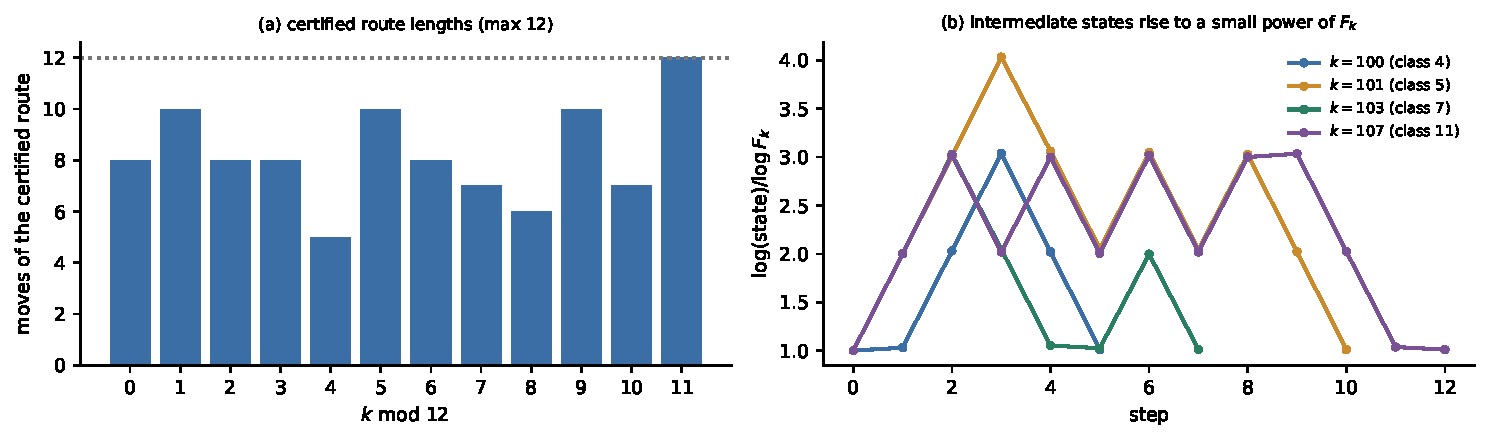
\includegraphics[width=\textwidth]{../figures/fig10_fibonacci.pdf}
\caption{(a) Lengths of the twelve certified routes. (b) Intermediate states for four values of $k$, on the scale $\log(\text{state})/\log F_k$.}\label{fig:fib}\end{figure}

\subsection{The twelve certified route families}\label{ssec:fibfamilies}
For each residue class of $k$ modulo $12$ the following lists give the moves of the certified route from $F_k$ to $F_{k+1}$, one move per line. A leading $+$ is a forward move $+N_i$ and a leading $-$ an inverse move $-N_i$; each label is an element $p_0(b)+p_1(b)\,a$ of the ring $O_\varepsilon$ of Proposition~\ref{prop:ring}, with $b=F_h$, $a=F_{h-1}$, $h=\lfloor k/2\rfloor$, and $\varepsilon=(-1)^h$ is the sign of the class. These are the certificates behind Theorem~\ref{thm:twelve}.
\needspace{14\baselineskip}\subsection*{Class $k\equiv 0\pmod{12}$ \quad ($\varepsilon=+1$, 8 moves)}
\begin{center}\renewcommand{\arraystretch}{1.35}\begin{tabular}{@{}r@{\quad}l@{}}\toprule
i & move $\pm N_i$ \\\midrule
1 & $+1$ \\
2 & $+(b \left(2 a + b\right))$ \\
3 & $+(4 \left(5 a b + 10 b^{2} + 1\right))$ \\
4 & $-(4 b \left(a + 2 b\right))$ \\
5 & $+(b \left(a + 2 b\right))$ \\
6 & $-(5 b^{2} + 4)$ \\
7 & $-(a b + 3 b^{2} + 1)$ \\
8 & $-1$ \\
\bottomrule\end{tabular}\end{center}

\needspace{14\baselineskip}\subsection*{Class $k\equiv 1\pmod{12}$ \quad ($\varepsilon=+1$, 10 moves)}
\begin{center}\renewcommand{\arraystretch}{1.35}\begin{tabular}{@{}r@{\quad}l@{}}\toprule
i & move $\pm N_i$ \\\midrule
1 & $+(a b + 3 b^{2} + 1)$ \\
2 & $+(a b + 2 b^{2} + 1)$ \\
3 & $+(2 a + 3 b)$ \\
4 & $+(2 a + 3 b + 1)$ \\
5 & $-(\frac{2 a + 3 b}{2})$ \\
6 & $-(a b + 2 b^{2} + 1)$ \\
7 & $-(a + b - 1)$ \\
8 & $+(\frac{a + 2 b - 1}{2})$ \\
9 & $-(a + 2 b)$ \\
10 & $-(3 a b + 4 b^{2} + 1)$ \\
\bottomrule\end{tabular}\end{center}

\needspace{14\baselineskip}\subsection*{Class $k\equiv 2\pmod{12}$ \quad ($\varepsilon=-1$, 8 moves)}
\begin{center}\renewcommand{\arraystretch}{1.35}\begin{tabular}{@{}r@{\quad}l@{}}\toprule
i & move $\pm N_i$ \\\midrule
1 & $+(b \left(2 a + b\right))$ \\
2 & $+(a b + 2 b^{2} - 1)$ \\
3 & $+(- b \left(a - 2 b\right))$ \\
4 & $+(4 \left(5 b^{2} + 1\right))$ \\
5 & $-(4 b^{2})$ \\
6 & $-(- 5 a b + 5 b^{2} - 1)$ \\
7 & $-(b \left(a + 3 b\right))$ \\
8 & $-(a b + 3 b^{2} - 1)$ \\
\bottomrule\end{tabular}\end{center}

\needspace{14\baselineskip}\subsection*{Class $k\equiv 3\pmod{12}$ \quad ($\varepsilon=-1$, 8 moves)}
\begin{center}\renewcommand{\arraystretch}{1.35}\begin{tabular}{@{}r@{\quad}l@{}}\toprule
i & move $\pm N_i$ \\\midrule
1 & $+(a b + 3 b^{2} - 1)$ \\
2 & $+(5 a b + 10 b^{2} - 1)$ \\
3 & $-(\left(b - 1\right) \left(b + 1\right))$ \\
4 & $+(4 \left(b - 1\right) \left(b + 1\right))$ \\
5 & $-(4 \left(5 b^{2} - 4\right))$ \\
6 & $-(\frac{3 a b + 4 b^{2} - 4}{2})$ \\
7 & $+(\frac{3 a b + 4 b^{2} - 4}{6})$ \\
8 & $-(\frac{3 a b + 4 b^{2} - 1}{3})$ \\
\bottomrule\end{tabular}\end{center}

\needspace{14\baselineskip}\subsection*{Class $k\equiv 4\pmod{12}$ \quad ($\varepsilon=+1$, 5 moves)}
\begin{center}\renewcommand{\arraystretch}{1.35}\begin{tabular}{@{}r@{\quad}l@{}}\toprule
i & move $\pm N_i$ \\\midrule
1 & $+1$ \\
2 & $+(b \left(2 a + b\right))$ \\
3 & $+(\frac{5 a b + 10 b^{2} + 1}{4})$ \\
4 & $-(5 b^{2} + 4)$ \\
5 & $-(a b + 3 b^{2} + 1)$ \\
\bottomrule\end{tabular}\end{center}

\needspace{14\baselineskip}\subsection*{Class $k\equiv 5\pmod{12}$ \quad ($\varepsilon=+1$, 10 moves)}
\begin{center}\renewcommand{\arraystretch}{1.35}\begin{tabular}{@{}r@{\quad}l@{}}\toprule
i & move $\pm N_i$ \\\midrule
1 & $+(a b + 3 b^{2} + 1)$ \\
2 & $+(5 b^{2} + 4)$ \\
3 & $+(5 \left(a b + 2 b^{2} + 1\right))$ \\
4 & $-(b^{2})$ \\
5 & $-(3 a b + 4 b^{2} - 1)$ \\
6 & $+(\frac{3 a b + 4 b^{2} - 1}{2})$ \\
7 & $-(\frac{5 b \left(a + b\right)}{2})$ \\
8 & $+(b \left(a + b\right))$ \\
9 & $-(5 b^{2} + 4)$ \\
10 & $-(3 a b + 4 b^{2} + 1)$ \\
\bottomrule\end{tabular}\end{center}

\needspace{14\baselineskip}\subsection*{Class $k\equiv 6\pmod{12}$ \quad ($\varepsilon=-1$, 8 moves)}
\begin{center}\renewcommand{\arraystretch}{1.35}\begin{tabular}{@{}r@{\quad}l@{}}\toprule
i & move $\pm N_i$ \\\midrule
1 & $+(b \left(2 a + b\right))$ \\
2 & $+(a b + 2 b^{2} - 1)$ \\
3 & $-(- \frac{a b - 2 b^{2} + 2}{2})$ \\
4 & $+(- \frac{a b - 2 b^{2} + 2}{4})$ \\
5 & $-(- \frac{b \left(a - 2 b\right)}{2})$ \\
6 & $+(- b \left(a - 2 b\right))$ \\
7 & $-(b^{2})$ \\
8 & $-(a b + 3 b^{2} - 1)$ \\
\bottomrule\end{tabular}\end{center}

\needspace{14\baselineskip}\subsection*{Class $k\equiv 7\pmod{12}$ \quad ($\varepsilon=-1$, 7 moves)}
\begin{center}\renewcommand{\arraystretch}{1.35}\begin{tabular}{@{}r@{\quad}l@{}}\toprule
i & move $\pm N_i$ \\\midrule
1 & $+(a b + 3 b^{2} - 1)$ \\
2 & $+(5 a b + 10 b^{2} - 1)$ \\
3 & $-(\frac{5 b^{2} - 4}{4})$ \\
4 & $-(\frac{3 a b + 4 b^{2} - 4}{2})$ \\
5 & $-1$ \\
6 & $+(\frac{3 a b + 4 b^{2} - 4}{6})$ \\
7 & $-(\frac{3 a b + 4 b^{2} - 1}{3})$ \\
\bottomrule\end{tabular}\end{center}

\needspace{14\baselineskip}\subsection*{Class $k\equiv 8\pmod{12}$ \quad ($\varepsilon=+1$, 6 moves)}
\begin{center}\renewcommand{\arraystretch}{1.35}\begin{tabular}{@{}r@{\quad}l@{}}\toprule
i & move $\pm N_i$ \\\midrule
1 & $+(b \left(2 a + b\right))$ \\
2 & $+(4 \left(5 a b + 10 b^{2} + 1\right))$ \\
3 & $-(4 b \left(a + 2 b\right))$ \\
4 & $+(b \left(a + 2 b\right))$ \\
5 & $-(5 b^{2} + 4)$ \\
6 & $-(a b + 3 b^{2} + 1)$ \\
\bottomrule\end{tabular}\end{center}

\needspace{14\baselineskip}\subsection*{Class $k\equiv 9\pmod{12}$ \quad ($\varepsilon=+1$, 10 moves)}
\begin{center}\renewcommand{\arraystretch}{1.35}\begin{tabular}{@{}r@{\quad}l@{}}\toprule
i & move $\pm N_i$ \\\midrule
1 & $+(a b + 3 b^{2} + 1)$ \\
2 & $+(a b + 2 b^{2} + 1)$ \\
3 & $-(2 a + 3 b - 1)$ \\
4 & $+(\frac{2 a + 3 b - 1}{2})$ \\
5 & $+(\frac{2 a + 3 b + 1}{2})$ \\
6 & $-(\frac{2 a + 3 b - 1}{4})$ \\
7 & $+(8 a b + 13 b^{2} + 3)$ \\
8 & $-(a b + 2 b^{2} + 1)$ \\
9 & $-(3 a b + 5 b^{2} + 1)$ \\
10 & $-(3 a b + 4 b^{2} + 1)$ \\
\bottomrule\end{tabular}\end{center}

\needspace{14\baselineskip}\subsection*{Class $k\equiv 10\pmod{12}$ \quad ($\varepsilon=-1$, 7 moves)}
\begin{center}\renewcommand{\arraystretch}{1.35}\begin{tabular}{@{}r@{\quad}l@{}}\toprule
i & move $\pm N_i$ \\\midrule
1 & $+1$ \\
2 & $+4$ \\
3 & $+(b \left(2 a + b\right))$ \\
4 & $+(\frac{5 \left(a b + 2 b^{2} - 1\right)}{4})$ \\
5 & $-(5 b^{2})$ \\
6 & $-4$ \\
7 & $-(a b + 3 b^{2} - 1)$ \\
\bottomrule\end{tabular}\end{center}

\needspace{14\baselineskip}\subsection*{Class $k\equiv 11\pmod{12}$ \quad ($\varepsilon=-1$, 12 moves)}
\begin{center}\renewcommand{\arraystretch}{1.35}\begin{tabular}{@{}r@{\quad}l@{}}\toprule
i & move $\pm N_i$ \\\midrule
1 & $+(a b + 3 b^{2} - 1)$ \\
2 & $+(5 a b + 10 b^{2} - 1)$ \\
3 & $-(5 b^{2} - 1)$ \\
4 & $+(\frac{5 b^{2} - 1}{4})$ \\
5 & $-(\frac{5 b^{2} + 1}{2})$ \\
6 & $+(3 a b + 5 b^{2} - 1)$ \\
7 & $-(\frac{3 a b + 5 b^{2} - 2}{2})$ \\
8 & $+(\frac{3 a b + 4 b^{2} - 1}{4})$ \\
9 & $+3$ \\
10 & $-(3 a b + 4 b^{2} + 2)$ \\
11 & $-(\frac{3 a b + 4 b^{2} - 1}{3})$ \\
12 & $-1$ \\
\bottomrule\end{tabular}\end{center}



\subsection{Small $k$ and the uniform bound}
For $2\le k\le29$ the exact distance was computed by bidirectional enumeration and a shortest path recorded (Table~\ref{tab:fibsmall}; independently recomputed here for $k\le25$, all values agreeing, and each stored path re-checked edge by edge for all $k\le29$).
\begin{table}[ht]\centering
{\footnotesize\begin{longtable}{@{}rcp{0.78\textwidth}@{}}\toprule
$k$ & $d(F_k,F_{k+1})$ & a shortest path\\\midrule\endhead
2 & 5 & $1 \to 4 \to 16 \to 100 \to 9 \to 2$ \\
3 & 4 & $2 \to 9 \to 48 \to 12 \to 3$ \\
4 & 4 & $3 \to 16 \to 162 \to 36 \to 5$ \\
5 & 2 & $5 \to 36 \to 8$ \\
6 & 5 & $8 \to 32 \to 128 \to 24 \to 196 \to 13$ \\
7 & 5 & $13 \to 196 \to 1792 \to 448 \to 84 \to 21$ \\
8 & 5 & $21 \to 192 \to 768 \to 3456 \to 648 \to 34$ \\
9 & 4 & $34 \to 136 \to 9522 \to 396 \to 55$ \\
10 & 5 & $55 \to 720 \to 4500 \to 32400 \to 8100 \to 89$ \\
11 & 5 & $89 \to 8100 \to 1800 \to 400 \to 36 \to 144$ \\
12 & 5 & $144 \to 900 \to 24336 \to 246402 \to 54756 \to 233$ \\
13 & 5 & $233 \to 54756 \to 246402 \to 17496 \to 142884 \to 377$ \\
14 & 6 & $377 \to 11700 \to 480000 \to 43200 \to 2420000 \to 4392 \to 610$ \\
15 & 5 & $610 \to 187272 \to 1216 \to 48672 \to 976144 \to 987$ \\
16 & 5 & $987 \to 3948 \to 3904576 \to 5646019600 \to 2553604 \to 1597$ \\
17 & 6 & $1597 \to 6388 \to 10214416 \to 368019400 \to 1559376 \to 103428 \to 2584$ \\
18 & 5 & $2584 \to 49248 \to 50626992 \to 12321 \to 480852 \to 4181$ \\
19 & 5 & $4181 \to 163172 \to 18766224 \to 208513600 \to 115456 \to 6765$ \\
20 & 5 & $6765 \to 385728 \to 47232 \to 69808928 \to 4630184 \to 10946$ \\
21 & 5 & $10946 \to 59929352 \to 2492336 \to 7928121600 \to 3560000 \to 17711$ \\
22 & 5 & $17711 \to 1611900 \to 358200 \to 5133006025 \to 821280964 \to 28657$ \\
23 & 6 & $28657 \to 821280964 \to 1852810219150 \to 507619200 \to 4145556800 \to 2690172 \to 46368$ \\
24 & 6 & $46368 \to 1161216 \to 26763264 \to 370028890000 \to 17576372275 \to 225300100 \to 75025$ \\
25 & 6 & $75025 \to 225300100 \to 9017932950 \to 112706100 \to 751862410000 \to 14736503236 \to 121393$ \\
26 & 6 & $121393 \to 63488772 \to 37322572996800 \to 75578228767641600 \to 16512612007500 \to 19290408200 \to 196418$ \\
27 & 5 & $196418 \to 38580423561 \to 136808280 \to 4382425236 \to 101004467344 \to 317811$ \\
28 & 5 & $317811 \to 1271244 \to 404017869376 \to 187919215512250000 \to 264432492900 \to 514229$ \\
29 & 6 & $514229 \to 264432492900 \to 40195501804086 \to 4363384860 \to 20102114997552 \to 692292225681 \to 832040$ \\
\bottomrule\end{longtable}}

\caption{Exact $\dist(F_k,F_{k+1})$ for $2\le k\le29$ with a shortest path.}\label{tab:fibsmall}\end{table}
\emph{Proof of Theorem~\ref{thm:fibonacci}.} For $k\ge20$ use Theorem~\ref{thm:twelve}: the route has at most $12$ moves. For $2\le k\le29$ use Table~\ref{tab:fibsmall}. \hfill$\square$
\begin{remark}[Interpretation]
Boundedness of $\dist$ is not special to Fibonacci numbers: ratio-matched pairs $(a,\lfloor\varphi a\rceil)$ behave similarly in the data of the earlier release. What is special is \emph{uniformity with an explicit certified formula}: one finite list of integer-valued label formulas, valid for infinitely many $k$ at once.
\end{remark}
